\chapter{Pruebas durante el desarrollo y corrección de errores}
Una de las etapas más importantes durante el desarrollo de una aplicación es la de la creación y ejecución de pruebas. Desde ir probando determinadas configuraciones en la creación de formularios, comprobaciones de la navegabilidad e interacción de componentes hasta comprobar la fluidez y los tiempos de carga.
\\Antes de sacar un proyecto a producción han de pasar por un testeo y eso sobre lo que tratará este último capítulo.

\section{Pruebas durante el desarrollo}
Las herramientas que han utilizado para la realización de pruebas durante el desarrollo del proyecto han sido tres:
\begin{itemize}
    \item \textbf{Postman}: Para poder realizar pruebas sobre la API.
    \item \textbf{Selenium}: Para poder realizar pruebas más que nada orientadas al envío de formularios.
    \item \textbf{Herramientas de Desarrollador de Google Chrome}: Para poder controlar la consola, algunos problemas de estilos y el envío y recibo de paquetes en la red.
\end{itemize}

\subsection{Postman}
Gracias a Postman se ha podido probar en este proyecto todas las interacciones que se pueden realizar con la API y el proxy configurado en Angular.
\begin{figure}[h]
    \centering
    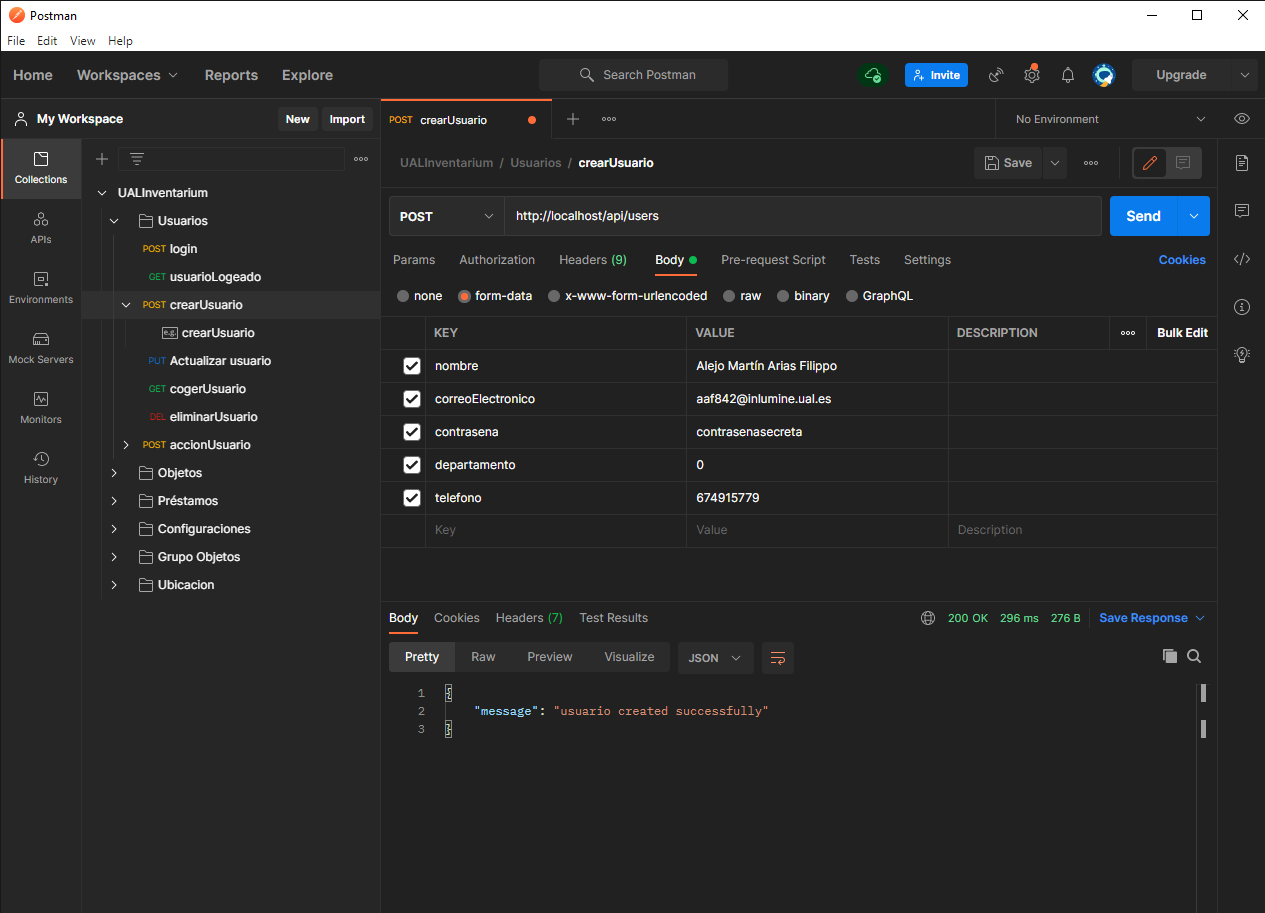
\includegraphics[scale=0.3,keepaspectratio]{../pruebas/postman_creation_user.png}
    \caption{Creando un usuario con Postman}\label{fig:postman-creation-user}
\end{figure}
Como puede comprobarse en la figura \ref{fig:postman-creation-user} se ha generado una solicitud POST para mandarla a la dirección \textit{/api/users} de la página web. Que a su vez la redirigirá al registro probando el proxy.
\\Se añaden los parámetros dentro del campo \textit{form-data} ubicado dentro de \textit{Body} que es la forma en la que se ha planificado el procesado de las peticiones.
\\Luego de pulsar en el botón \textit{Send} puede comprobarse que se manda la solicitud porque llega una respuesta que de la API, en este caso: \textit{`message': `usuario created successfully'}
\\Un punto bastante a favor que presenta Postman es que el conjunto de solicitudes que tengas se almacena en tu usuario por lo que al cambiar de dispositivo estas solicitudes se siguen manteniendo.
\\Otra herramienta que tiene incorporada esta aplicación te permite capturar solicitudes que salgan de un determinado puerto. Aparte de capturarlas, interpreta en su totalidad las estructuras de estas y puede comprobarse si se ha cometido algún fallo al mandar cualquier tipo de solicitud desde la página.

\subsection{Selenium}
Gracias a la herramienta de grabación que aporta Selenium se han realizado bastantes pruebas en la página web.
\\Para poder utilizar la herramienta se ha hecho desde Google Chrome instalando la siguiente \href{https://chrome.google.com/webstore/detail/selenium-ide/mooikfkahbdckldjjndioackbalphokd}{\textbf{extensión}}.
\\Luego de instalarla hay que dirigirse a la lista de complementos del navegador y seleccionar la aplicación. Se pulsará en crear nuevo proyecto y la aplicación pedirá una \textit{url} para empezar a grabar pruebas. Se añadirá la url \textit{http://localhost/register} para poder automatizar el proceso de registro.
\\Al empezar la grabación se abrirá una nueva ventana de Google Chrome y se completarán los datos como un proceso normal de registro pulsando finalmente en \textit{Registrarse}.
\\La prueba que se ha generado puede verse en la figura \ref{fig:registro-usuario-selenium}
\begin{figure}[h]
    \centering
    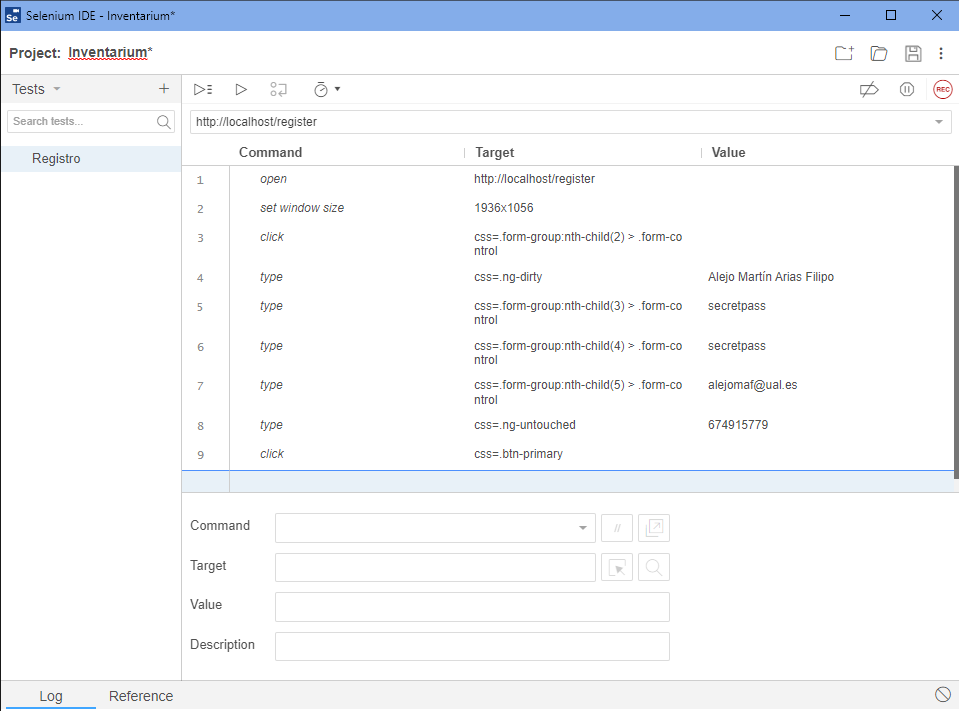
\includegraphics[scale=0.40,keepaspectratio]{../pruebas/registro_usuario_selenium.png}
    \caption{Registro de un usuario con Selenium}\label{fig:registro-usuario-selenium}
\end{figure}
\subsection{Herramientas de Desarrollador de Google Chrome}
Las Herramientas de Desarrollador de Google han sido utilizadas en todas las fases del desarrollo de la aplicación. Desde las más tempranas hasta las más tardías.
\\El navegador Google Chrome brinda un conjunto de herramientas muy completo. Las tres que más se han utilizado han sido:
\begin{itemize}
    \item \textbf{Elements}: Aquí pueden verse los elementos presentes en pantalla. Disponem también de un inspector que permite pulsar sobre un elemento y localizarlo dentro de la estructura HTML que presenta el documento. También permite poder editar los estilos con los que se esté trabajando y ver los cambios en tiempo real. Estos no se aplican al documento pero ayudan en gran medida a realizar arreglos de diseño.
    \item \textbf{Console}: Desde aquí pueden verse las salidas de consola que da la aplicación. En Angular para poder emitir señales en la consola se utiliza \textit{console.log(``Elemento que quiera emitirse'')}. Desde aquí pueden verse fallos que haya devuelto la aplicación y poder actuar en medida.
    \item \textbf{Network}: Esta sección es de gran ayuda porque desde aquí se pueden ver todos los paquetes entrantes y salientes desde el punto de vista del cliente.
\end{itemize}
\begin{figure}[h]
    \centering
    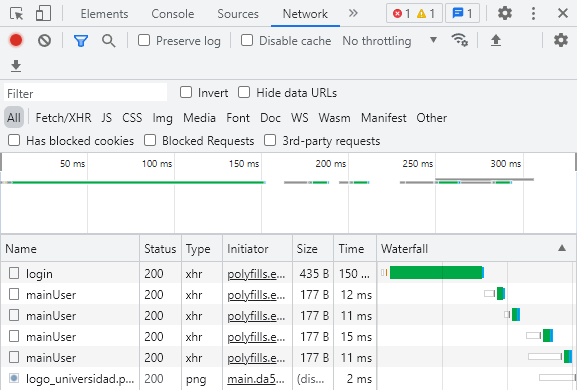
\includegraphics[scale=0.6,keepaspectratio]{../pruebas/network_dev_tools_chrome.png}
    \caption{Sección \textit{Network} dentro de las herramientas de desarrollador de Google Chrome}
\end{figure}
\section{Corrección de errores}
Para poder realizar esta sección se han ido recopilando las correcciones más significativas que ha sufrido el proyecto.

\subsection{Cambio de la base de datos}
Cuando se estaba realizando la construcción del sitio web con la base de datos y la API ya programadas se pidió crear un nuevo tipo de objeto. Este objeto serían los kits.
\\Los kits consistían en un grupo de objetos que en realidad eran un conjunto de otros objetos. Poder remodelar la página para adaptar la lógica de los kits fue bastante complicado pero la solución bastante buena.
\\En un principio se iban a implementar dos nuevas tablas a la base de datos, una que se llamara \textbf{Kit} y otra \textbf{ObjetoKit}. Esto hubiera modificado la mayoría de consultas de generación de préstamos y suponía un aumento de la complejidad de la aplicación bastante grande. Había que distinguir en cada consulta si un elemento era un grupo de objetos o un kit.
\\Un tiempo después se comprobó que no hacía falta implementar un elemento del tipo Kit, ya que esta funcionalidad la cubría grupo de objeto.
\\El formato terminó consistiendo en que un grupo de objetos contenía dos tipos de parámetros diferentes: objetos u objeto kit. Los objeto kit eran los objetos de los que estaba compuesto el kit, en caso de serlo. Mientras que los objetos era el número de elementos con sus distintos atributos que podía tener.

\subsection{Cambios de solicitudes}
En las etapas intermedias del proyecto cuando estaba siendo realizando el proceso de creación de un grupo de objetos se tuvo que hacer una readaptación.
\\El problema ocurría a la hora de estar subiendo imágenes a la base de datos y es que para poder procesar y enviar estas imágenes se tuvieron que usar campos de formularios.
\\No había problema hasta que los plugins que había de procesamiento de formularios no eran compatibles con el que se tenía para poder procesar solicitudes en formato json.
\\Así que por las imágenes tanto de los grupos de objetos como las de los objetos de kit se tuvo que cambiar todo el repertorio de solicitudes que había sido creado para la creación, modificación, actualización y eliminación de elementos para adaptarlos con un formato de formularios.

\subsection{Conexión entre máquinas de Docker Compose}
Resulta que al configurar la API con la base de datos había que esperar a que la base de datos se encendiera, como se ha explicado en la configuración del documento de docker compose.
\\Esta estaba mandando constatemente solicitudes TCP al puerto 3306 que es el que usaba la base de datos y posteriormente cuando se intentaba conectar daba un error de conexión.
\\Al analizar los errores en la terminal se vió que la base de datos había mandado un mensaje que decía que no había sido posible conectar con ella porque las credenciales eran del estilo \textit{`user':`unnauthenticated'} y \textit{`password':`unset'}.
\\La solución fue, como se ha señalado anteriormente en este documento: que, para poder realizar una conexión con una máquina en un entorno local de Docker desplegado con Docker Compose hay que referenciar la máquina con el nombre con la que se había creado. Quedando así:
\begin{verbatim}
const connection = await mysql.createConnection({
    host: 'db',
    user: 'ualinventarium',
    password: 'secretpassword',
    database: 'ualinventarium',
    port: '3306'
});
\end{verbatim}